 \section{Durchführung}
\label{sec:Durchführung}

\subsection{Versuchsaufbau}

Der grundlegende Versuchsaufbau ist in Abbildung \ref{fig:versuchsaufbau} zu
sehen. Neben den für das Arbeiten des Helium-Neon Lasers relevanten Bauteilen
ist außerdem noch ein Justierlaser gegeben, damit die gesamte Apparatur
bequem auf die optische Achse justiert werden kann. Der auskoppelnde Spiegel
hat einen Transmissionskoeffizienten von
\begin{align}
  T \approx \SI{1.5}{\percent} - \SI{1.8}{\percent}
\end{align}
und einen Krümmungsradius von etwa
\begin{align}
  r_{\text{out}} = \SI{1400}{\milli\meter}.
\end{align}
Für die Einzelmessungen, die im folgenden Abschnitt besprochen werden,
stehen noch weitere Bauteile zur Verfügung.

\begin{figure}
  \centering
  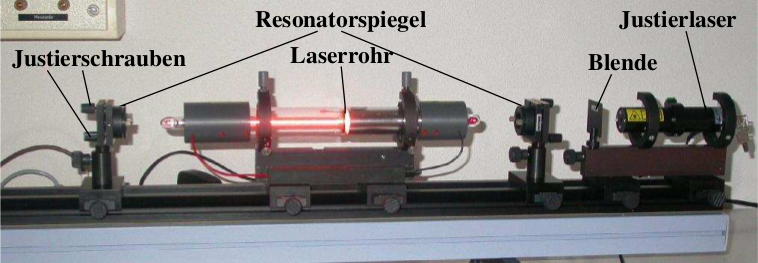
\includegraphics[height=4.3cm]{Pics von Buddy/versuchsaufbau.png}
  \caption{Grundlegender Versuchsaufbau für den Betrieb des Helium-Neon Lasers.
  Je nach Messung können weitere optische Bauteile hinzugefügt werden \cite{anleitung}.}
  \label{fig:versuchsaufbau}
\end{figure}

\subsection{Messung}

Bei allen Justageschritten mit dem Helium-Neon Laser ist es unabdingbar eine Schutzbrille
zu tragen, da die Laserleistung hoch genug ist um erhebliche Schäden an den Augen
hervorzurufen.

\begin{enumerate}
  \item Im ersten Schritt wird der Helium-Neon Laser mit Hilfe des Justierlasers justiert.
  Dazu werden nacheinander die relevanten Bauteile, darunter die beiden Spiegel und das
  Lasermedium mit Brewsterfenstern, auf die Schiene gestellt und so justiert, dass die
  Rückreflexe wieder auf einem Fadenkreuz, welches sich direkt vor dem Justierlaser befindet,
  landen. Ist die Vorjustage erfolgreich, so kann der Helium-Neon Lasers eingeschaltet
  werden, indem die Stromstärke auf $I = \SI{6.5}{\milli\ampere}$ gesetzt wird. Nach einer
  kurzen Warmlaufzeit und vorsichtigem Nachjustieren an den Resonatorspiegeln sollte
  das rote Laserlicht erkennbar sein.
  \item Als nächstes wird mit Hilfe eines Polarisationsfilters und einer Photodiode
  die Intensität in Abhängigkeit von der Polarisatoreinstellung gemessen. Die genaue
  Einstellung des Brewsterfensters ist hier nicht relevant, aber das gemessene
  Intensitätsmaximum sollte ungefähr bei einer Polarisatoreinstellung parallel
  zur Einfallsebene des Brewsterfensters maximal sein.
  \item Im dritten Schritt werden die $\text{TEM}_{00}$- und die $\text{TEM}_{01}$-Mode des
  Lasers ausgemessen. Dazu wird eine defokussierende Linse hinter dem auskoppelnden
  Spiegel platziert um das Laserintensitätsbild zu vergrößern. Durch Verschieben der
  Photodiode dahinter kann ein Intensitätsbild erstellt werden. Bei der Ausmessung
  der $\text{TEM}_{01}$-Mode muss wie bereits erwähnt zusätzlich noch eine Modenblende
  innerhalb des Resonators platziert werden um die $\text{TEM}_{00}$-Mode auszublenden.
  \item Anschließend wird mit Hilfe eines Spaltgitters, welches hinter dem auskoppelnden
  Spiegel platziert wird, die Wellenlänge des Lasers vermessen. Dazu werden die Abstände
  der resultierenden Intensitätsmaxima auf einem Schirm hinter dem Beugungsobjekt
  ausgemessen.
  \item Im fünften Schritt werden die longitudinalen Moden ausgemessen wie bereits in
  den theoretischen Grundlagen in Abschnitt \ref{sec:long} erklärt. Dazu trifft der
  Laserstrahl erneut auf eine Photodiode und das detektierte Signal anschließend in ein
  FFT-Gerät, wo es fouriertransformiert wird. Die Abstände der Frequenzpeaks können
  am Gerät abgelesen werden.
  \item Schließlich wird noch eine Stabilitätsmessung für einen konkaven und einen planaren Spiegel
  durchgeführt. Dazu wird für eine steigende Resonatorlänge der Laser zum Lasen gebracht falls
  möglich. Die Resonatorlänge kann dabei mit einem Maßband ermittelt werden.
\end{enumerate}

Im folgenden Kapitel werden die Ergebnisse dieser Messungen präsentiert und ausgewertet.
